\chapter{Konzeption und Design der Todo-App}
\section{Architektur der Anwendung}
Die Todo-App ist als eine mehrschichtige Architektur konzipiert, die eine klare Trennung der Verantwortlichkeiten zwischen den verschiedenen Schichten sicherstellt. Diese Architektur umfasst die folgenden Schichten:

\begin{itemize}
	\item \textbf{Präsentationsschicht}: Diese Schicht besteht aus REST-Controllern, die HTTP-Anfragen entgegennehmen und HTTP-Antworten zurückgeben. Sie interagiert mit der Service-Schicht, um Geschäftslogik zu implementieren.
	\item \textbf{Service-Schicht}: Diese Schicht enthält die Geschäftslogik der Anwendung. Sie validiert die Daten und ruft die entsprechenden Methoden der Repository-Schicht auf.
	\item \textbf{Repository-Schicht}: Diese Schicht besteht aus JPA-Repositories, die für die Datenzugriffslogik verantwortlich sind. Sie interagiert mit der MySQL-Datenbank, um Daten zu speichern und abzurufen.
	\item \textbf{Sicherheitsschicht}: Diese Schicht nutzt Spring Security, um Authentifizierung und Autorisierung zu implementieren. JWT (JSON Web Tokens) wird verwendet, um die Benutzersitzungen zu verwalten.
	\item \textbf{Datenbank-Schicht}: Diese Schicht besteht aus einer MySQL-Datenbank, in der alle Daten der Anwendung gespeichert werden.
\end{itemize}

\section{Datenmodell und Datenbankdesign}

\subsection{Entwurf des Datenmodells}
Das Datenmodell der Todo-App umfasst mehrere Entitäten, um die Beziehungen zwischen Benutzern und ihren Aufgaben zu verwalten. Die Hauptentitäten sind User und Todo.

\textbf{User Entität}

Die User-Entität repräsentiert einen Benutzer der Anwendung und enthält folgende Attribute:

\begin{itemize}
	\item id: Ein eindeutiger Bezeichner für jeden Benutzer.
	\item username: Der Benutzername, den der Benutzer zur Anmeldung verwendet.
	\item password: Das verschlüsselte Passwort des Benutzers.
\end{itemize}

Die User-Entität wird als Java-Klasse implementiert und mit JPA-Anmerkungen versehen, um die Zuordnung zur Datenbank zu erleichtern.

\begin{lstlisting}
	@Entity
	public class User {
		
		@Id
		@GeneratedValue(strategy = GenerationType.IDENTITY)
		private Long id;
		
		@Column(unique = true, nullable = false)
		private String username;
		
		@Column(nullable = false)
		private String password;
		
		// Getter und Setter
	}
\end{lstlisting}
	
\textbf{Todo Entität}

Die Todo-Entität repräsentiert eine Aufgabe und enthält folgende Attribute:

\begin{itemize}
	\item id: Ein eindeutiger Bezeichner für jede Todo.
	\item title:  Der Titel der Todo.
	\item description: Eine Beschreibung der Todo.
	\item dueDate: Das Fälligkeitsdatum der Todo.
	\item completed: Ein boolescher Wert, der angibt, ob die Todo abgeschlossen ist.
	\item user: Eine Beziehung zum Benutzer, der die Todo erstellt hat.
\end{itemize}

Die Todo-Entität wird als Java-Klasse implementiert und mit JPA-Anmerkungen versehen, um die Zuordnung zur Datenbank zu erleichtern.

\begin{lstlisting}
	@Entity
	public class Todo {
		
		@Id
		@GeneratedValue(strategy = GenerationType.IDENTITY)
		private Long id;
		
		@Column(nullable = false)
		private String title;
		
		@Column
		private String description;
		
		@Column
		private LocalDate dueDate;
		
		@Column(nullable = false)
		private boolean completed;
		
		@ManyToOne
		@JoinColumn(name = "user_id", nullable = false)
		private User user;
		
		// Getter und Setter
	}
\end{lstlisting}

\subsection{Projektanforderungen an die Datenbank}

Das Projekt stellt spezifische Anforderungen an die Datenbank, die durch MySQL erfüllt werden:

\begin{itemize}
	
	\item \textbf{Open source}: Die Datenbank muss open source sein, da keine Kosten für die Verwendung der Datenbank anfallen dürfen. My SQL bietet eine MySQL Community Edition an, die open source ist \cite{noauthor_mysql_nodate}.
	\item \textbf{Datenintegrität und Konsistenz}: Die Datenbank muss in der Lage sein, Daten in einer strukturierten und konsistenten Weise zu speichern. MySQL gewährleistet dies durch die Verwendung relationaler Tabellen und die Unterstützung von Transaktionen \cite{noauthor_mysql_nodate} .
	%\item \textbf{Skalierbarkeit}: Das Projekt muss in der Lage sein, mit wachsendem Datenvolumen und steigender Benutzeranzahl zu skalieren.
	\item \textbf{Sicherheit}: Der Schutz sensibler Daten ist von entscheidender Bedeutung. MySQL bietet umfassende Sicherheitsfunktionen wie SSL-Verschlüsselung, Datenmaskierung und Authentifizierungs-Plugins, um die Datensicherheit zu gewährleisten \cite{noauthor_mysql_nodate} .
	\item \textbf{Performance}: Das Projekt erfordert schnelle Datenverarbeitungszeiten, um eine reibungslose Benutzererfahrung zu gewährleisten. MySQL bietet eine hohe Geschwindigkeit und Effizienz bei der Verarbeitung großer Datenbanken\cite{noauthor_was_2022}.
	\item \textbf{Flexibilität und Integration}: Die Datenbank muss flexibel genug sein, um mit verschiedenen Programmiersprachen und Technologien integriert zu werden. MySQL bietet eine breite Unterstützung für verschiedene Systeme und Schnittstellen \cite{noauthor_was_2022}.
	\item \textbf{Benutzerfreundlichkeit}: Eine einfache Installation und Verwaltung der Datenbank ist erforderlich, um den Entwicklungsprozess zu optimieren. MySQL ist benutzerfreundlich und bietet zahlreiche Verwaltungstools, die die Bedienung erleichtern \cite{noauthor_was_2022}.
\end{itemize}

Diese Anforderungen des Projekts werden durch die funktionalen und technischen Merkmale von MySQL umfassend abgedeckt, was die Entscheidung für MySQL als Datenbanklösung rechtfertigt.


\subsection{Datenbankdesign}

Das Datenbankdesign umfasst zwei Tabellen: users und todos. Die Struktur der Tabellen ist wie folgt:

Tabelle users
\begin{itemize}
	\item id (BIGINT, AUTO\_INCREMENT, PRIMARY KEY)
	\item username (VARCHAR, NOT NULL, UNIQUE)
	\item password (VARCHAR, NOT NULL)
\end{itemize}

Tabelle todos
\begin{itemize}
	\item id (BIGINT, AUTO\_INCREMENT, PRIMARY KEY)
	\item title (VARCHAR, NOT NULL)
	\item description (TEXT)
	\item dueDate (DATE)
	\item completed (BOOLEAN, NOT NULL)
	\item user\_id (BIGINT, FOREIGN KEY)
\end{itemize}

Durch diese Struktur wird sichergestellt, dass jede Aufgabe eindeutig einem Benutzer zugeordnet ist. Diese Beziehung ermöglicht es, dass Benutzer nur ihre eigenen Todos sehen und verwalten können.

\section{User Interface Design}

\subsection{Gestaltung der Benutzeroberfläche}

Die Benutzeroberfläche der Todo-App ist so gestaltet, dass sie intuitiv und benutzerfreundlich ist. Die Anwendung besteht aus mehreren Ansichten, die jeweils spezifische Funktionen bereitstellen:

\begin{itemize}
	\item \textbf{/IndexView}: Die Startseite der Anwendung siehe Abbildung \ref{UI_index}. Diese Seite bietet zwei Hauptoptionen: "`Log in"' und "`Sign up"'. Dies ermöglicht neuen Benutzern die Registrierung und bestehenden Benutzern die Anmeldung.
	
	\begin{figure}[h]
		\centering
		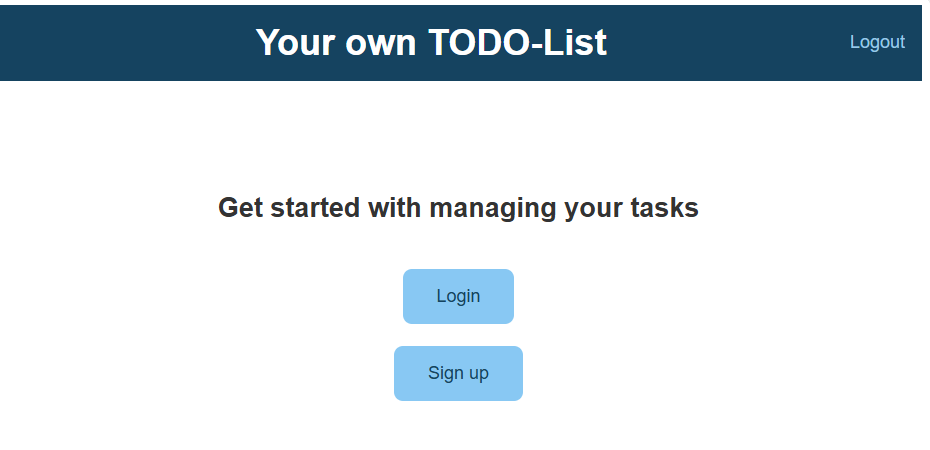
\includegraphics[clip,width=0.75\linewidth]{images/index.png}
		\caption[User Interface Design der Startseite]{User Interface Design der Startseite [Eigene Darstellung]}
		\label{UI_index}
	\end{figure}	
	
	\item \textbf{/LoginView}: Die Anmeldeseite siehe Abbildung \ref{UI_logIn}. Hier können Benutzer ihren Benutzernamen und ihr Passwort eingeben, um auf ihre persönlichen Aufgabenlisten zuzugreifen. Ein Link zur Registrierung ist ebenfalls vorhanden.
	
	\begin{figure}[h]
		\centering
		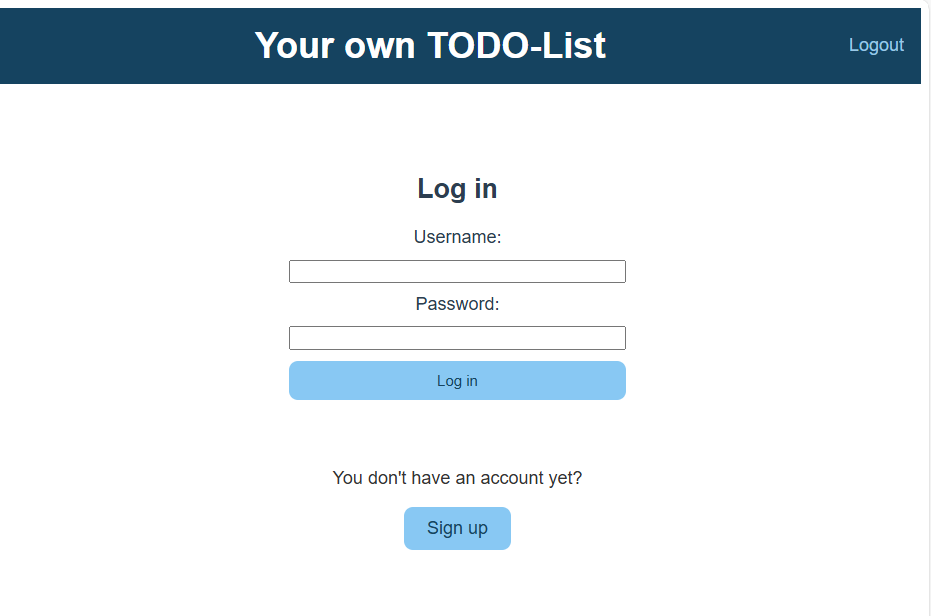
\includegraphics[clip,width=0.75\linewidth]{images/logIn.png}
		\caption[User Interface Design der Anmeldeseite]{User Interface Design der Anmeldeseite [Eigene Darstellung]}
		\label{UI_logIn}
	\end{figure}	
	
	\item \textbf{/RegisterView}: Die Registrierungsseite siehe Abbildung \ref{UI_signUp}. Neue Benutzer können hier ein Konto erstellen, indem sie ihren Benutzernamen, ihr Passwort und die Bestätigung des Passworts eingeben. Ein Link zur Anmeldung für bestehende Benutzer ist ebenfalls verfügbar.
	
	\begin{figure}[h]
		\centering
		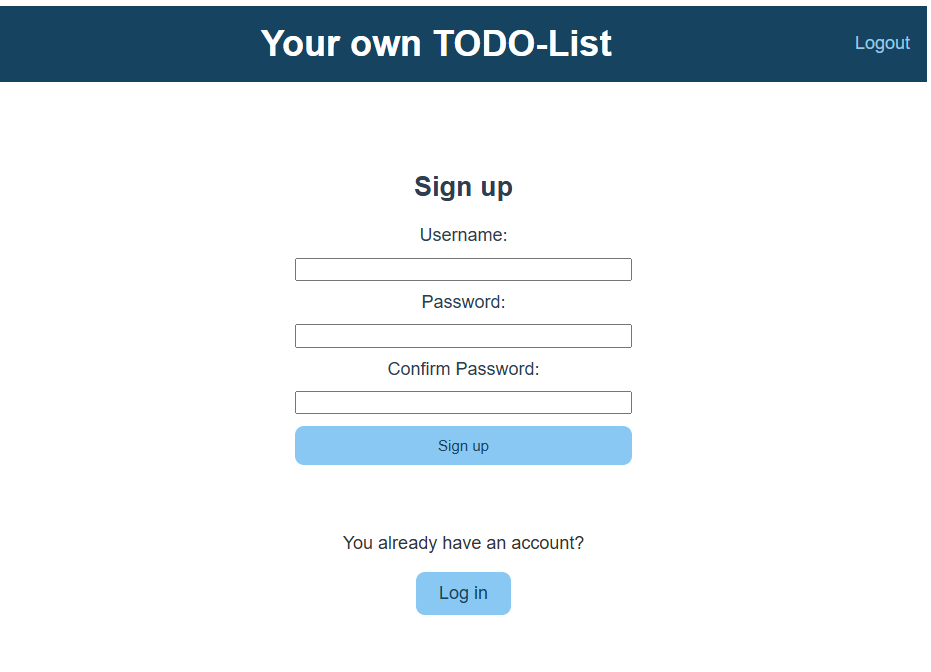
\includegraphics[clip,width=0.75\linewidth]{images/signUp.png}
		\caption[User Interface Design der Registrierungsseite]{User Interface Design der Registrierungsseite [Eigene Darstellung]}
		\label{UI_signUp}
	\end{figure}	
	
	\item \textbf{/HomeView}: Die Hauptseite nach der Anmeldung siehe Abbildung \ref{UI_home}. Diese Seite zeigt die Aufgabenliste des angemeldeten Benutzers. Benutzer können neue Aufgaben erstellen, vorhandene Aufgaben bearbeiten oder löschen.
	
	\begin{figure}[h]
		\centering
		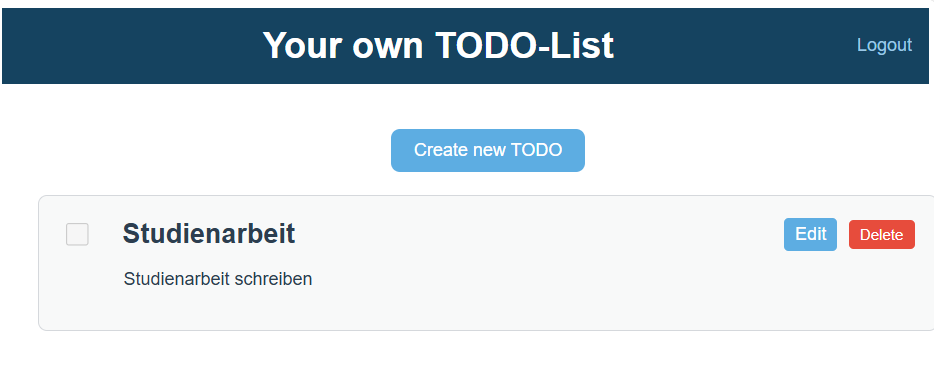
\includegraphics[clip,width=0.75\linewidth]{images/home.png}
		\caption[User Interface Design der Hauptseite]{User Interface Design der Hauptseite [Eigene Darstellung]}
		\label{UI_home}
	\end{figure}	
	
	\item \textbf{/NewTodoForm}: Diese Seite bietet ein Formular zum Erstellen einer neuen Todo siehe Abbildung \ref{UI_newTodo}.
	% TODO
	
	\begin{figure}[h]
		\centering
		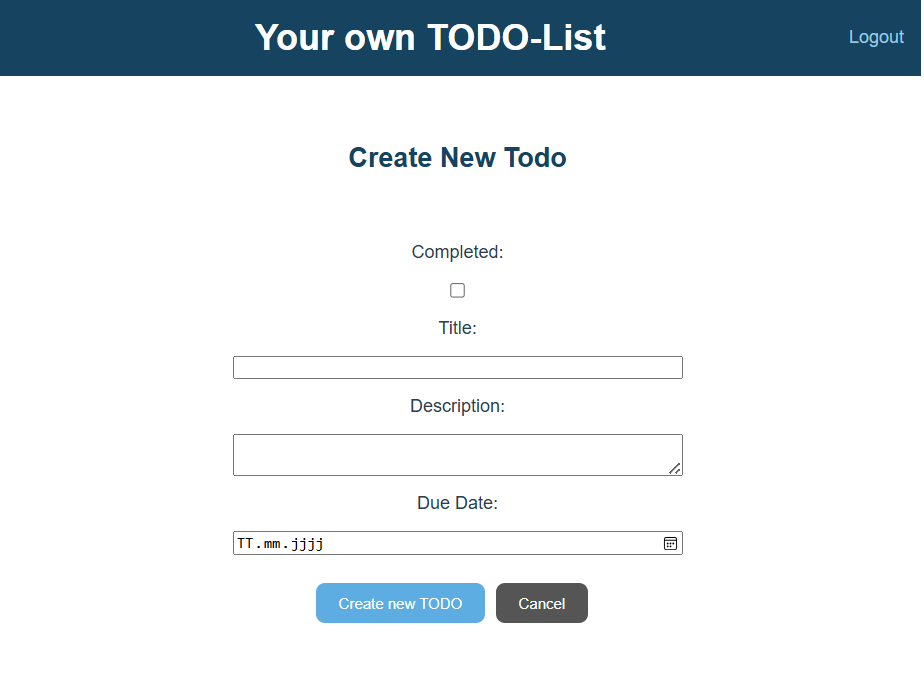
\includegraphics[clip,width=0.75\linewidth]{images/newTodo.png}
		\caption[User Interface Design der Ansicht zum Erstellen einer neuen Todo]{User Interface Design der Ansicht zum Erstellen einer neuen Todo [Eigene Darstellung]}
		\label{UI_newTodo}
	\end{figure}
	
	\item \textbf{/TodoDetailView}: Die Detailansicht einer spezifischen Todo siehe Abbildung \ref{UI_idTodo}. Diese Seite ermöglicht es Benutzern, die Details einer ausgewählten Todo zu bearbeiten.
	
	\begin{figure}[h]
		\centering
		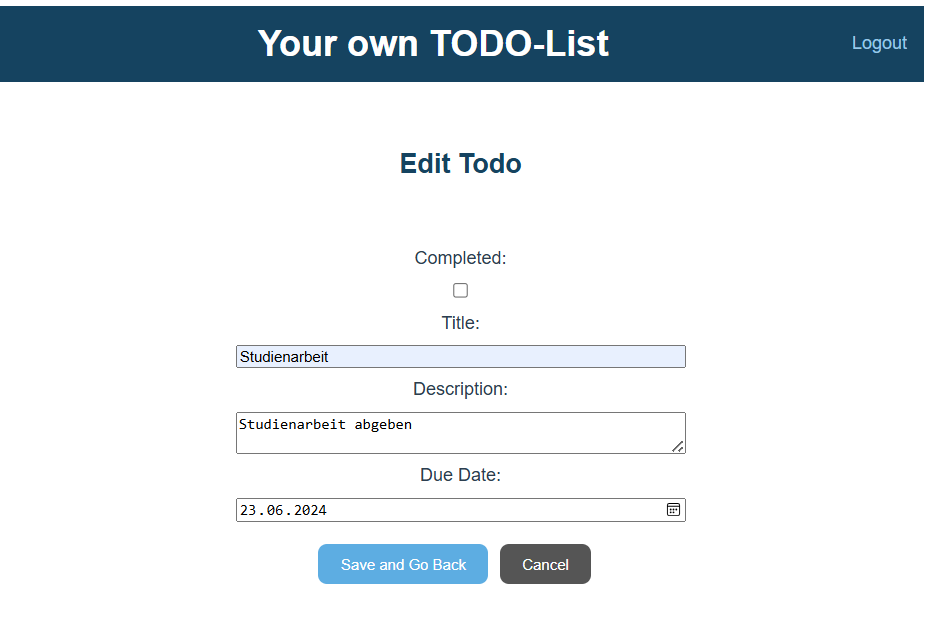
\includegraphics[clip,width=0.75\linewidth]{images/idTodo.png}
		\caption[User Interface Design der Detailansicht zum Bearbeiten]{User Interface Design der Detailansicht [Eigene Darstellung]}
		\label{UI_idTodo}
	\end{figure}	
	
\end{itemize}

Jede Seite hat ein konsistentes Layout mit einem zentralen Header. Der Header ist als eine Komponente in der \textbf{/HeaderBar} definiert. Er enthält das Logo "`Your own TODO-List"' und die Logout-Option, abhängig davon, ob der Benutzer angemeldet ist.

\subsection{Berücksichtigung von Usability-Prinzipien}

Das User Interface Design der Todo-App folgt mehreren grundlegenden Usability-Prinzipien nach Jakob Nielsen \cite{nielsen_10_nodate}, um sicherzustellen, dass die Anwendung einfach zu bedienen und effizient ist:

\begin{enumerate}
	\item \textbf{Sichtbarkeit des Systemstatus}: Die App hält den Benutzer stets über den aktuellen Status und die Ergebnisse ihrer Aktionen informiert. Beispielsweise werden Änderungen an Aufgaben sofort angezeigt und erfolgreiche Anmeldungen führen direkt zur Hauptseite mit der Aufgabenliste.
	\item \textbf{Übereinstimmung zwischen System und realer Welt}: Die Anwendung verwendet Begriffe und Konzepte, die den Benutzern vertraut sind. Schaltflächen und Symbole sind intuitiv und leicht verständlich, was die Bedienung erleichtert.
	\item \textbf{Benutzerkontrolle und Freiheit}: Benutzer können Aktionen rückgängig machen. Es gibt deutlich sichtbare Optionen zum Abbrechen von Aktionen, um Fehlaktionen leicht korrigieren zu können.
	\item \textbf{Konsistenz und Standards}: Das Layout und das Design der Benutzeroberfläche sind auf allen Seiten der Anwendung konsistent. Dies erleichtert den Benutzern das Verständnis und die Navigation durch die App.
	%\item \textbf{Fehlervermeidung}: Die Anwendung enthält Sicherheitsabfragen und Bestätigungsdialoge, um unbeabsichtigte Aktionen zu verhindern. Beispielsweise wird vor dem Löschen einer Aufgabe eine Bestätigung eingeholt.
	% TODO: mit rein nehmen, wenn es sicherheitsabfragen gibt
	\item \textbf{Wiedererkennung statt Erinnerung}: Die Benutzeroberfläche macht alle wichtigen Optionen und Funktionen sichtbar, damit Benutzer sie leicht wiedererkennen können, anstatt sich an sie erinnern zu müssen. Wichtige Elemente wie Schaltflächen und Eingabefelder sind prominent platziert und leicht zu finden. Der Einsatz von Farben und Schriftgrößen hilft, die Aufmerksamkeit der Benutzer auf wichtige Aktionen und Informationen zu lenken.
	%\item \textbf{Flexibilität und Effizienz der Nutzung}: 
	\item \textbf{Ästhetik und minimalistisches Design}: Das Design ist einfach und übersichtlich gehalten, um die Benutzerfreundlichkeit zu erhöhen. Unnötige Elemente wurden vermieden, um Ablenkungen zu minimieren und den Fokus auf die Hauptfunktionen der Anwendung zu legen.
	\item \textbf{Hilfe beim Erkennen, Diagnostizieren und Beheben von Fehlern}: Fehlernachrichten sind in einfacher Sprache verfasst und bieten klare Hinweise zur Problemlösung. Beispielsweise wird bei einer fehlerhaften Anmeldung eine verständliche Fehlermeldung angezeigt und mögliche Lösungen vorgeschlagen.
	% TODO: Fehlermeldungen und Lösungsmöglichkeiten
	%\item \textbf{Hilfe und Dokumentation}: Obwohl die App so gestaltet ist, dass sie intuitiv bedienbar ist, steht den Benutzern bei Bedarf eine leicht durchsuchbare Hilfedokumentation zur Verfügung. Diese enthält konkrete Anleitungen zur Durchführung von Aufgaben.
\end{enumerate}




